\documentclass[times,specification,annotation]{itmo-student-thesis}
\linespread{1.4}

%% Опции пакета:
%% - specification - если есть, генерируется задание, иначе не генерируется
%% - annotation - если есть, генерируется аннотация, иначе не генерируется
%% - times - делает все шрифтом Times New Roman, собирается с помощью xelatex
%% - languages={...} - устанавливает перечень используемых языков. По умолчанию это {english,russian}.
%%                     Последний из языков определяет текст основного документа.

%% Делает запятую в формулах более интеллектуальной, например:
%% $1,5x$ будет читаться как полтора икса, а не один запятая пять иксов.
%% Однако если написать $1, 5x$, то все будет как прежде.
\usepackage{icomma}

%% Один из пакетов, позволяющий делать таблицы на всю ширину текста.
\usepackage{tabularx}

\usepackage[hidelinks]{hyperref}
%% Данные пакеты необязательны к использованию в бакалаврских/магистерских
%% Они нужны для иллюстративных целей
%% Начало
\usepackage{tikz}
\usetikzlibrary{arrows}
\usepackage{filecontents}
\begin{filecontents}{bachelor-thesis.bib}
@online{ big-graphs-future-arxiv,
    year        = {2020},
    title       = {The Future is Big Graphs! A Community View on Graph Processing Systems},
    author      = {Sherif Sakr and Angela Bonifati and Hannes Voigt and Alexandru Iosup and Khaled Ammar and Renzo Angles},
    url         = {https://arxiv.org/abs/2012.06171},
    langid      = {english}
}

@online{ graph-db-scale,
    year        = {2022},
    title       = {Graph Database Scalability},
    author      = {Neo4j},
    url         = {https://neo4j.com/product/neo4j-graph-database/scalability/},
    langid      = {english}
}

@online{ saner,
    year        = {2020},
    title       = {Ultra-Large-Scale Repository Analysis via Graph Compression},
    author      = {Paolo Boldi and Antoine Pietri and Sebastiano Vigna and Stefano Zacchiroli},
    url         = {https://upsilon.cc/~zack/research/publications/saner-2020-swh-graph.pdf},
    langid      = {english}
}

@online{ scale-cost,
    year        = {2015},
    title       = {Scalability! But at what COST?},
    author      = {Frank McSherry and Michael Isard and Derek G. Murray},
    url         = {https://www.usenix.org/system/files/conference/hotos15/hotos15-paper-mcsherry.pdf},
    langid      = {english}
}

@online{ gremlin,
    year        = {2022},
    title       = {Gremlin Query Language},
    author      = {{Apache TinkerPop}},
    url         = {https://tinkerpop.apache.org/gremlin.html},
    langid      = {english}
}

@online{ swh-main-page,
    year        = {2022},
    title       = {Software Heritage},
    author      = {{Software Heritage}},
    url         = {https://www.softwareheritage.org/},
    langid      = {english}
}

@online{ swh-intern,
    year        = {2022},
    title       = {TinkerPop Gremlin backend for WebGraph (internship)},
    author      = {{Software Heritage}},
    url         = {https://wiki.softwareheritage.org/wiki/TinkerPop_Gremlin_backend_for_WebGraph_(internship)},
    langid      = {english}
}

@online{ webgraph,
    year        = {2022},
    title       = {WebGraph},
    author      = {WebGraph},
    url         = {https://webgraph.di.unimi.it/},
    langid      = {english}
}

@online{ tinkerpop-enabled,
    year        = {2022},
    title       = {Data System Providers},
    author      = {{Apache TinkerPop}},
    url         = {https://tinkerpop.apache.org/providers.html},
    year        = {2022},
    langid      = {english}
}

@online{ tinkerpop,
    year        = {2022},
    title       = {Apache TinkerPop},
    author      = {{Apache TinkerPop}},
    url         = {https://tinkerpop.apache.org/},
    langid      = {english}
}

@online{ git,
    year        = {2022},
    title       = {Git},
    author      = {{Git}},
    url         = {https://git-scm.com/},
    langid      = {english}
}

@online{ swh-dataset,
    year        = {2022},
    title       = {Dataset - Software Heritage},
    author      = {{Software Heritage}},
    url         = {https://docs.softwareheritage.org/devel/swh-dataset/graph/dataset.html},
    langid      = {english}
}

@online{ swh-api,
    year        = {2022},
    title       = {Graph RPC API - Software Heritage},
    author      = {{Software Heritage}},
    url         = {https://docs.softwareheritage.org/devel/swh-graph/api.html},
    langid      = {english}
}

@online{ vigna-bidir,
    year        = {2022},
    title       = {Add BidirectionalImmutableGraph to hold a graph and its transpose},
    author      = {{vigna}},
    url         = {https://github.com/vigna/webgraph-big/commit/debeb714e1392c5d171fea784115de63c1086170},
    year        = {2022},
    langid      = {english}
}

@online{ fastutil,
    year        = {2022},
    title       = {fastutil},
    author      = {{fastutil}},
    url         = {https://fastutil.di.unimi.it},
    year        = {2022},
    langid      = {english}
}

\end{filecontents}
%% Конец

%% Указываем файл с библиографией.
\addbibresource{bachelor-thesis.bib}

\begin{document}

\studygroup{M34391}
\title{Реализация TinkerPop инфраструктуры для WebGraph}
\author{Стародубцев Андрей Игоревич}{Стародубцев А.И.}
\supervisor{Аксенов Виталий Евгеньевич}{Аксенов В.Е.}{PhD, науки}{главный научный сотрудник Университета ИТМО}
\publishyear{2022}
%% Дата выдачи задания. Можно не указывать, тогда надо будет заполнить от руки.
\startdate{31}{января}{2022}
%% Срок сдачи студентом работы. Можно не указывать, тогда надо будет заполнить от руки.
\finishdate{15}{мая}{2022}
%% Дата защиты. Можно не указывать, тогда надо будет заполнить от руки.
\defencedate{9}{июня}{2022}

\addconsultant{Zacchiroli Stefano}{HDR, Full Professor}

\secretary{Штумпф С.А.}

%% Задание
%%% Техническое задание и исходные данные к работе
\technicalspec{Требуется реализовать инфраструктуру фреймворка для обработки графов Apache TinkerPop, позволяющую обрабатывать графы, сжатые фреймворком WebGraph. Это позволит обрабатывать графы очень больших размеров (десятки миллиардов вершин) при помощи экспрессивного доменно-ориентированного языка для обхода графов Gremlin. Для реализации требуется разработать программный слой, связывающий модели данных TinkerPop и WebGraph, реализовать структурные интерфейсы TinkerPop для WebGraph, добавить поддержку различных подходов к хранению свойств вершин/ребер, оценить производительность реализации на представляющих интерес запросах в конкретном домене (архив репозиториев Software Heritage), найти и исправить узкие места.}

%%% Содержание выпускной квалификационной работы (перечень подлежащих разработке вопросов)
\plannedcontents{TinkerPop - фреймворк изначально направленный на использование в графовых базах данных. При реализации для сжатых графов потребуется максимально оптимизировать слой, связывающий два фреймворка, чтобы не препятствовать масштабируемости.

Поскольку WebGraph не предоставляет единого способа хранения свойств вершин/ребер, необходимо разработать абстракции, которые позволят TinkerPop получать доступ и вычислять значения этих свойств во время исполнения запросов.

Для анализа производительности потребуется  реализовать на Gremlin ряд содержательных запросов в определенном домене, и замерить время их выполнения. Сравнение с нативными реализациями запросов позволит оценить практическую пользу реализации.}

%%% Исходные материалы и пособия
\plannedsources{\begin{enumerate}
    \item документация фреймворка для обработки графов Apache TinkerPop;
    \item документация фреймворка для сжатия графов WebGraph;
    \item документация Software Heritage.
\end{enumerate}}


%% ------ Конец части из ИСУ

%%% Цель исследования
\researchaim{Добавление возможности исполнения Gremlin запросов на графах, сжатых фреймворком WebGraph.}

%%% Задачи, решаемые в ВКР
\researchtargets{
\begin{enumerate}
    \item реализация интерфейсов TinkerPop, позволяющих исполнять Gremlin запросы на графах, сжатых с использованием WebGraph;
    \item создание универсального механизма доступа к хранимым свойствам вершин и ребер, позволяющего использовать Gremlin запросы, опирающиеся на наличие/значения свойств;
    \item проведение анализа производительности реализации и сравнение с нативными реализациями запросов;
\end{enumerate}
}

%%% Использование современных пакетов компьютерных программ и технологий
\addadvancedsoftware{Фреймворк \texttt{Apache TinkerPop}}{Список использованных источников}

%%% Краткая характеристика полученных результатов
\researchsummary{
Разработана библиотека, позволяющая осуществлять немодифицирующие Gremlin запросы к любым графам, сжатым фреймворком WebGraph. Библиотека включает в себя поддержку различных источников свойств/вершин ребер, а также возможность определять собственные механизмы доступа к свойствам. Сформулирован ряд запросов в домене архивации данных систем контроля версий репозиториев с открытым исходным кодом, и проведен анализ производительности библиотеки на этих запросах.
}

%%% Гранты, полученные при выполнении работы
\researchfunding{}

%%% Наличие публикаций и выступлений на конференциях по теме выпускной работы
\researchpublications{}

%% Эта команда генерирует титульный лист и аннотацию.
\maketitle{Бакалавр}

%% Оглавление
\tableofcontents

%% Макрос для введения. Совместим со старым стилевиком.
\startprefacepage

Графовое представление данных встречается все чаще \cite{big-graphs-future-arxiv}, а увеличение размеров таких графов приводит к необходимости использовать системы, которые справляются с масштабируемостью. Для графов малых/средних размеров могут использоваться графовые базы данных, предоставляющие достаточную производительность, а также широкие возможности для анализа данных с помощью запросов, сформулированных на специальных доменно-ориентированных языках, таких как Gremlin \cite{gremlin}. В случае больших графов (десятки миллиардов вершин, сотни миллиардов ребер) решением является сжатие графов. Фреймворк WebGraph \cite{webgraph} является единственным подобным решением и позволяет добиться хорошей производительности, в свою очередь, в отличие от графовых баз данных, требуя заметно меньше ресурсов \cite{graph-db-scale, scale-cost, saner}. Однако в данный момент такой подход предоставляет мало возможностей для анализа данных, поскольку способы доступы к вершинам и ребрам сжатого графа весьма лимитированы, и реализация запросов осуществляется вручную на каждый запрос, так как поддержки доменно-ориентированных языков для запросов WebGraph не предоставляют. Именно с такой проблемой столкнулась команда Software Heritage \cite{swh-main-page, swh-intern}, использующая фреймворк WebGraph для сжатия графа репозиториев \cite{saner}, и при консультации которой велась работа над данной задачей.

Суммируя, в данный момент пользователям, работающими с данными в графовом представлении, требуется выбрать: либо использовать графовую базу данных, чтобы получить возможность исполнять запросы на экспрессивном доменно-ориентированном языке, либо использовать сжатое представление графа, пожертвовав экспрессивностью языка запросов, взамен получив эффективную работу с памятью, и как следствие эффективное исполнение запросов.
Цель данной работы --- предоставить возможность пользоваться обоими преимуществами: формулировать запросы на экспрессивном доменно-ориентированном языке, сохранив превосходство сжатия графов в исполнении запросов. Для этого планируется добавить поддержку Gremlin запросов для графов, сжатых фреймворком WebGraph.

Первая глава содержит описание предметной области, а также постановку задачи. Во второй главе рассматриваются шаги, необходимые для достижения поставленной цели, а также описан подход к верификации решения. В третьей главе подробно описываются детали реализации основной части решения. Четвертая глава показывает, каким образом был проведен анализ производительности решения, и какие результаты были выявлены.

%% Начало содержательной части.
\chapter{Обзор предметной области}

\startrelatedwork
Многие задачи предполагают хранение данных в графовом представлении. Если пользователю необходимо извлечь некую информацию из этих данных, ему потребуется определить и выполнить некий запрос для этой структуры данных. Запрос может быть реализован нативно, то есть с использованием непосредственно методов лежащей в основе структуры. Такой подход не является гибким, так как требует ручной реализации на каждый отдельный случай. Альтернативой являются доменно-ориентированные языки для обхода графов, позволяющие формулировать гибкие запросы. В данной главе будет подробно описана данная предметная область, приведена решаемая проблема и аргументирована ее актуальность на конкретном примере.

\section{Язык для обхода графов Gremlin}

Gremlin - доменно-ориентированный язык для обхода графов, разработанный компанией Apache \cite{gremlin}. Является самым популярным языком подобного рода с открытым исходным кодом, о чем свидетельствует его широкая поддержка множеством графовых баз данных \cite{tinkerpop-enabled}. Действительно, основной областью использования Gremlin являются графовые базы данных, и это становится заметно при рассмотрении возможностей Gremlin. Несмотря на это, Gremlin позволяет гибко формулировать любые запросы для любых графов, вне зависимости от лежащей в основе системы.

\begin{lstlisting}[float=!h,caption={Пример запроса на Gremlin},label={lst1}]
g.V().has('code','LED')
     .repeat(out().simplePath())
     .until(has('code','SVO'))
     .path().by('code').limit(10)
\end{lstlisting}

В Gremlin запросах пользователь может опираться как на структуру графа, то есть сами вершины и ребра, так и на свойства вершин и ребер. Свойства это дополнительная информация, хранящаяся в вершинах и ребрах. Примером такой информации может быть название аэропорта для графа рейсов, а примером свойства ребра может являться расстояние между аэропортами. 

Для исполнения запросов Gremlin использует фреймворк Apache TinkerPop \cite{tinkerpop}. Любая система имеет возможность реализовать инфраструктуру Apache TinkerPop (англ. TinkerPop-enabled system), что позволит исполнять в ней Gremlin запросы. Примерами подобных систем являются описанные ранее графовые базы данных.

\section{Ограничения графовых баз данных}

Предоставляя стандартную поддержку Gremlin, графовые базы данных дают возможность исполнять Gremlin запросы в своей системе - требуется лишь адаптировать свою систему под одну из таких баз данных. Такое решение хорошо подходит для графов малых/средних размеров. Однако, когда речь идет о больших графах (десятки миллиардов вершин, сотни миллиардов ребер), требуется масштабируемое решение. Графовые базы данных масштабируются за счет распределенных систем \cite{graph-db-scale}, на создание и поддержание которых требуются большие ресурсы.

\section{Сжатие графов}

Другим подходом к обеспечению хорошей производительности при работе с большими графами является сжатие графов. Такой подход позволяет существенно сократить размер графа в памяти. Это в свою очередь дает возможность разместить весь граф в оперативной памяти одного компьютера \cite{saner}, что существенно повышает эффективность доступа к графу, и позволяет анализировать его без использования распределенной системы. Стоит отметить, что под сжатием графа понимается сжатие именно его структуры, а не свойств. Единственным решением подобного рода с открытым исходным кодом является фреймворк WebGraph \cite{webgraph}.

\section{Ограничения WebGraph}

WebGraph позволяет эффективно хранить граф за счет сжатия его структуры, однако WebGraph не представляет поддержки Gremlin. Таким образом любой запрос к подобному графу требует реализации вручную, а WebGraph предоставляет весьма ограниченные способы доступа к структуре графа.
Помимо этого, WebGraph не предоставляет универсального способа для работы со свойствами вершин и ребер, работа с ними во многом становится обязанностью пользователя. При этом многие представляющие интерес запросы зависят от значений свойств вершин и ребер.

\section{Объединения преимуществ подходов}

todo

\section{Software Heritage}

Software Heritage - компания, занимающаяся архивированием данных систем контроля версий репозиториев с открытым исходным кодом. Архив представляет собой единый граф. Графовое представление обусловлено устройством распределенных систем контроля версий, таких как git \cite{git}, базирующихся на дереве хешей (точнее на ациклическом ориентированном графе). Структура графа приведена на рисунке~\ref{fig1}.

\begin{figure}[!h]
\caption{Структура архива Software Heritage}\label{fig1}
\centering
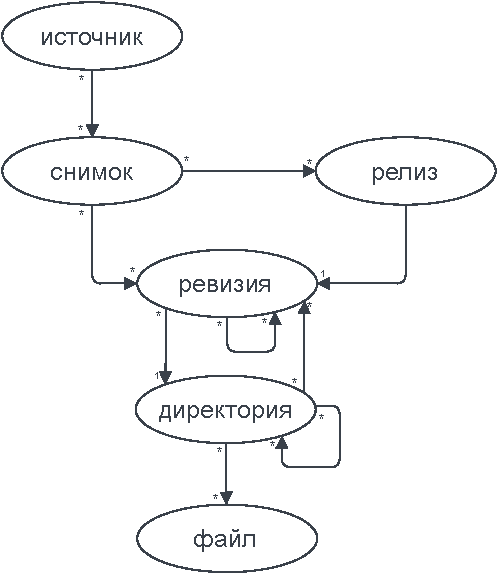
\includegraphics{img/swh-graph-structure.pdf}
\end{figure}

Единый граф архива содержит более двадцати миллиардов вершин и более двухсот тридцати миллиардов ребер \cite{swh-dataset}. При таком крупном размере графа эффективное исполнение запросов на нем возможно при сжатии структуры графа, что позволяет разместить весь граф в менее чем ста гигабайтах оперативной памяти \cite{saner}. При этом для сжатия структуры используется описанный ранее фреймворк WebGraph.

Архив Software Heritage содержит большое количество информации, анализ которой может представлять интерес. Веб-сервер Software Heritage предоставляет доступ к фиксированному набору запросов на графе, позволяющих анализировать информацию, хранящуюся в графе. \cite{swh-api}. Как было описано ранее, WebGraph предоставляет возможность осуществлять запросы к сжатому графу только в нативном виде - непосредственно используя методы, предоставляющие доступ к структуре графа. Это означает, что каждый предоставленный веб-сервером запрос потребовал непосредственной реализации на стороне сервера, а реализация нового запроса потребует вновь использовать лимитированные методы WebGraph. Для того, чтобы упростить реализацию новых запросов к графу Software Heritage, а также стандартизировать подход к их реализации (вместо изучения методов WebGraph и реализации поверх них, может быть использован стандартный доменно-ориентированный язык), команда хочет изучить возможность использования языка Gremlin для этих нужд. В случае успеха это позволит обрабатывать большой граф Software Heritage c удобством экспрессивного высокоуровнего языка, при этом сохранив эффективность исполнения запросов, достигаемую сжатием графа \cite{swh-intern}.

\section{Проверка производительности}

Поскольку TinkerPop предоставляет широкие возможности для обхода графов и в основном направлен на работу с графовыми базами данных, а WebGraph в свою очередь предоставляет весьма лимитированный набор методов, предоставляющих доступ к структуре графа, фокусируясь на оптимизации памяти, следует проверить, не внесет ли их связка проблем с производительностью, и убедиться, что решение имеет практическую пользу. Для этого потребуется провести анализ производительности, собрав данные об эффективности исполнения запросов, сравнив их с нативным реализациями.

\section{Постановка задачи}

Целью работы является реализация TinkerPop инфраструктуры для фреймворка для сжатия графов WebGraph. Это позволит выполнять сложные запросы на больших графах, используя язык Gremlin. Кроме того, необходимо добавить возможность указывать сторонние источники свойств вершин/ребер. После этого требуется сформулировать ряд запросов, анализ производительности исполнения которых покажет, насколько данный подход применим на практике.

\finishrelatedwork

\chapterconclusion
В первой главе была описана предметная область работы. Было показано, какая проблема существует, приведен пример случая, в котором решение этой проблемы будет актуально, а также разобраны альтернативные способы решения, и почему они в этом случае не подходят.

\chapter{Предлагаемый подход к решению}

В данной главе будет описана общая структура решения, проведено разбиение на подзадачи, подробнее описаны детали каждой подзадачи. 

\section{Разбиение на подзадачи}

Исходя из постановки задачи можно выделить при отдельные подзадачи:

\begin{enumerate}
    \item Реализовать интерфейсы Apache TinkerPop, превращающие WebGraph в TinkerPop-enabled систему
    \item Реализовать возможность указывать источники и способы доступа к свойствам вершин/ребер, для использования этих свойств в запросах
    \item Провести анализ производительности данной реализации
\end{enumerate}

Далее каждая из подзадач по отдельности будет рассмотрена подробнее.

\section{Реализация TinkerPop для WebGraph}

В данном разделе описывается общая архитектуры решения, а также  связка представлений графа в TinkerPop и WebGraph.

\subsection{Общая архитектура}

Поскольку данная реализация нацелена на случай, в котором пользователь уже использует фреймворк WebGraph, а значит располагает представлением сжатого графа, и уже имеет возможность исполнять на нем нативные запросы, однако хочет получить возможность исполнять запросы и на Gremlin, следует рассматривать реализацию как библиотеку, получающую в том или ином виде сжатый WebGraph граф, и предоставляющую таким образом возможность исполнять на нем запросы на Gremlin, делегируя описанные выше методы лежащему в основе сжатому графу, с добавлением требуемой пред- и пост-обработки аргументов и результатов.

\subsection{Структурные интерфейсы и методы TinkerPop}

Как было описано ранее, для получения возможности исполнять Gremlin запросы в собственной системе, требуется реализовать интерфейсы фреймворка Apache TinkerPop. Конкретнее, нужно реализовать интерфейсы пакета \texttt{/structure}, которые представляют абстракции для основных примитивов графовой модели - граф, вершина, ребро. Также, в этом пакете содержатся интерфейсы и методы для работы со свойствами, которые будут подробнее разобраны в следующем разделе.

Рассмотрим основные интерфейсы пакета \texttt{/structure}:

\begin{itemize}
    \item \texttt{Graph} - основной интерфейс графа. Экземпляр позволяет получать доступ к вершинам и ребрам по их идентификатору, либо ко всем вершинам и ребрам графа;
    \item \texttt{Vertex} - интерфейс вершины графа. Позволяет получить входящие и исходящие вершины и ребра, а также доступные свойства по их ключу;
    \item \texttt{Edge} - интерфейс ребра графа. Позволяет получить входящие и исходящие вершины, а также доступные свойства по их ключу;
    \item \texttt{Property} - интерфейс свойства вершины и ребра. Предоставляет доступ к значениям свойств;
\end{itemize}

Помимо описанных методов, TinkerPop поддерживает группы методов, поддержка которых реализовываться не будет:

\begin{itemize}
    \item Модифицирующие запросы - TinkerPop поддерживает запросы, модифицирующие граф. В данной реализации такие методы поддерживаться не будут, так как WebGraph не предоставляет возможности модифицировать граф во время работы с ним;
    \item Метасвойства вершин - TinkerPop поддерживает свойства вершин, являющиеся полноценными элементами графа, то есть имеющих свой уникальный идентификатор и свойства. В данной реализации такая возможность поддерживаться не будет, так как стандартной поддержки как мета-, так и обычных свойств вершин WebGraph не предоставляет.
    \item Специфичные для графовых баз данных методы - TinkerPop поддерживает методы, связаны со случаем использования в графовой базе данных, например \texttt{transaction()}. В данной реализации такая возможность поддерживаться не будет, так как в описываемом случае реализация основывается не на графовой базе данных.
\end{itemize}

Не стоит считать, что наличие подобных ограничений описываемого случая и как следствие отсутствие реализации указанных групп методов означает недостаточную совместимость TinkerPop и WebGraph. Как упоминалось ранее, несмотря на то, что TinkerPop действительно в большей мере направлен на работу с графовыми базами данных, где указанные группы методов оправданы, TinkerPop является фреймворком общего назначения для любых графовых систем, и отсутствие реализации указанных групп методов является ожидаемым, что подтверждается наличием стандартных исключений для каждой описанной ранее группы методов, информирующих об отсутствии реализации этой группы в данной системе.

\subsection{Отличия примитивов в WebGraph и TinkerPop}

Как было описано выше TinkerPop предоставляет абстракции для вершин и ребер, и работает с их экземплярами. WebGraph в свою очередь, предоставляет доступ только к вершинам, ссылаясь на их уникальный числовой идентификатор - индекс. Располагая индексом вершины можно получить итератор по индексам вершин-соседей. При этом отдельной абстракции для ребер в WebGraph нет. Это позволяет эффективно работать со структурой графа в памяти, однако усложняет работу с ней пользователю. Отличие в представлениях этих примитивов означает, что для реализации прослойки потребуется создавать объекты-обертки. Здесь можно рассмотреть два подхода:
\begin{enumerate}
    \item Сопоставить каждой вершине или ребру в WebGraph единственный объект, который будет возвращаться при любом доступе к данной вершине.
    \item Возвращать временные объекты при доступе к данной вершине или ребру - нет гарантии, что два различных запроса к одной вершине или ребру вернут один и тот же объект, однако гарантируется, что объекты будут равны и будут обладать одинаковыми свойствами.
\end{enumerate}

Первый вариант подразумевает создание единого реестра объектов, для получения гарантии идентичности возвращаемых объектов при различных запросах. Учитывая цель сохранить преимущество в использовании памяти, получаемое за счет сжатия графа, этот подход не является лучшим выбором, так как создает дополнительную нагрузку на память, которая при участии в обходе достаточного числа вершин, станет существенной проблемой.
Второй подход в свою очередь удобен своей гибкостью. Оставляя возможность создавать новые объекты при каждом новом обращении к вершине, он не исключает возможности внесения оптимизаций, для уменьшения общего числа аллокаций новых объектов.

\section{Работа со свойствами вершин и ребер графа}

Вершины и ребра в графе могут обладать свойствами. Примером свойства вершины может быть название аэропорта для графа рейсов, а свойством ребра может являться расстояние между аэропортами.
Многие запросы к графовой структуре данных представляют интерес именно в привязке к свойствам и их значениям, так как без их учета запрос может опираться только на структуру графа. Примером запроса на графе рейсов, зависящего от свойств вершин, может являться самый ранний рейс по выбранному направлению. В данном случае время вылета будет свойством вершины, обозначающей рейс.

\subsection{Свойства в TinkerPop}

Gremlin предоставляет возможность формулировать запросы, зависящие от свойств. Свойства устроены как пара ключ-значение, где ключ является строкой, а значение объектом. Gremlin позволяет как проверять наличие свойства с данным ключом у данной вершины или ребра, так и получать  значение свойства, а также использовать это значение, например для фильтрации.

\begin{lstlisting}[float=!h,caption={Пример запроса на Gremlin, зависящего от свойств},label={lst2}]
g.V().where(values('terminals').is(gt(3)))
\end{lstlisting}

TinkerPop в свою очередь предоставляет интерфейс \texttt{Property}, который используется для получения доступа к свойствам данной вершины или ребра. Имеется возможность как получить доступ ко всем доступным свойствам вершины или ребра, так и к конкретным свойствам, предоставив список ключей этих свойств. Этот список будет являться фильтром для доступных у данной вершины или ребра свойств.

Помимо свойств, TinkerPop также вводит понятие <<меток>>. Вершины и ребра могут обладать единственной строковой меткой. Так как метка единственна, для получения доступа к ней не требуется предоставлять ключ.

\begin{figure}[!h]
\caption{Архитектура свойств в TinkerPop}\label{fig2}
\centering
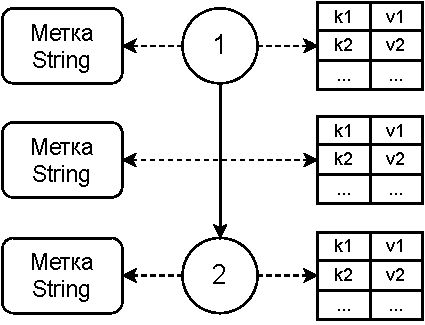
\includegraphics{img/tinker-props.pdf}
\end{figure}

\subsection{Свойства в WebGraph}

WebGraph - фреймворк, сжимающий графы с точки зрения их структуры. WebGraph предоставляет единственный способ работы со свойствами --- по индексу вершины можно получить как индексы ее соседей, так и <<помеченных>> соседей, то есть пару из индекса соседа и <<метки>>.
Эти метки можно считать свойством ребра из изначальной вершины в соседа. Для каждого ребра можно хранить единственный объект метку. В остальном работа со свойствами перекладывается на пользователя, в частности свойства вершин, хранение нескольких свойств для ребер.

\begin{figure}[!h]
\caption{Архитектура свойств в WebGraph}\label{fig3}
\centering
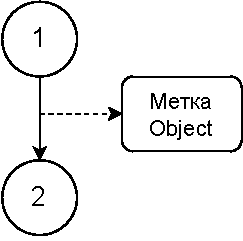
\includegraphics{img/webgraph-props.pdf}
\end{figure}

Тем не менее, хранение свойств вершин и ребер, помимо самой структуры графа, является важной элементом работы с графом, ведь как обсуждалось выше, запросы зачастую представляют интерес именно в привязке к свойствам. Поэтому существует ряд стандартных практик, использующихся для хранения и получения доступа к свойствам при работе с WebGraph.
К примеру для свойств вершин может использоваться сериализация массива примитивных значений, в котором индекс в массиве соответствует индексу вершины, а значение по индексу --- значению свойства для соответствующей вершины. Для того, чтобы пользователь имел возможность удобным образом задавать способ доступа к свойствам вершин и ребер, следует реализовать ряд классов, позволяющих как использовать стандартные методы хранения свойств, так и пользовательские способы хранения свойств.

\section{Анализ производительности реализации}

TinkerPop предоставляет широкие возможности для обхода графов, а также в основном используется в графовых базах данных. WebGraph в свою очередь фокусируется на достижении малого отпечатка в памяти, и используется в том случае, когда эффективность и минимальные накладные расходы критически необходимы.
При связке этих двух фреймворков могут возникнуть проблемы с производительностью --- требуется как сохранить малый отпечаток в памяти, достигаемый сжатием графа, так и оценить, не становятся ли критическими накладные расходы, которые появляются при адаптации WebGraph к TinkerPop.

Чтобы провести анализ производительности предлагается выбрать конкретный набор данных, представленный в виде графа. Следует определить ряд запросов, представляющих на нем интерес, после чего реализовать данные запросы на языке Gremlin, и, используя сжатое WebGraph представление данного графа и разработанную связку, исполнить данные запросы, проанализировав результаты по ряду метрик, таких как:

\begin{itemize}
    \item время выполнения;
    \item используемая память;
    \item число вершин/ребер, затронутых в процессе исполнения;
    \item число результатов;
\end{itemize}

Подобный анализ позволит оценить потерю в эффективности, вызванную разработанной связкой, и сделать выводы о практической применимости решения.

\chapterconclusion
В этой главе были подробнее рассмотрены конкретные шаги, необходимые для достижения поставленной задачи. Описаны основные интерфейсы WebGraph и TinkerPop, отличия в моделях свойств. Кроме того был описан подход к верификации решения.

\chapter{Реализация решения}

Фреймворк WebGraph реализован на языке Java, и так как решение нацелено на случай, в котором пользователь уже использует WebGraph, и желает получить возможность исполнять на доступном графе Gremlin запросы, решение также было реализовано на языке Java. TinkerPop также реализован на языке Java, что упрощает разработку связки двух фреймворков.

\section{Реализация TinkerPop}

Ранее были описаны интерфейсы и методы, предоставляемые TinkerPop, реализация которых позволяет исполнять в ней Gremlin запросы (англ. TinkerPop-enabled system). Согласно конвенции, реализации этих интерфейсов должны именоваться из двух частей: название системы, и название интерфейса в качестве суффикса. В качестве названия системы естественным образом было решено использовать \texttt{WebGraph}. Далее эти интерфейсы и их реализации будут рассмотрены подробнее. 

\subsection{WebGraphGraph}

Интерфейс \texttt{Graph} является основной точкой входа TinkerPop. Согласно конвенции его реализация для определенной системы должна содержать публичный статический метод (или несколько методов), возвращающий экземпляр этого класса, и этот метод должен использоваться для создания объектов интерфейса \texttt{Graph}.
Для связки с WebGraph этот метод должен получать в качестве параметра класс, предоставляющий доступ к сжатому графу. На момент начала работы единственным подходящим классом был \texttt{ImmutableGraph}, позволяющий обходить граф в одном направлении.
Поскольку TinkerPop позволяет обходить граф как в прямом, так и в обратном направлении ребер, после консультации в командой WebGraph, во фреймворк был добавлен новый класс \texttt{BidirectionalImmutableGraph} \cite{vigna-bidir}, позволяющий получать не только соседей по направлению ребер, но и соседей в обратном направлении todo(uml successors predecessors). Именно этот класс будет использоваться как основная точка доступа к структуре сжатого графа, а методы TinkerPop делегируются этому классу.

Помимо создания графа, интерфейс \texttt{Graph} позволяет получать доступ к вершинам и ребрам графа по их идентификаторам, либо ко всем вершинам или ребрам.

\subsubsection{Получение вершин}

Доступ к вершинам в TinkerPop осуществляется через метод \texttt{vertices(Object... vertexIds)}, возвращающий итератор по вершинам с данными индексами, либо итератор по всем вершинам, если массив предоставленных индексов пустой.
Так как индексы вершин в WebGraph это числа типа \texttt{Long}, ожидается, что будут предоставлены идентификаторы именно этого типа.
Для предоставленных индексов возвращаются объекты-обертки над ними класса \texttt{WebGraphVertex}, описанного ниже.
Если массив индексов пустой, обертки возвращаются над индексами, полученными методом \texttt{nodeIterator()} класса \texttt{ImmutableGraph}, возвращающем итератор по всем вершинам графа.

\subsubsection{Получение ребер}

Доступ к ребрам в TinkerPop осуществляется аналогично вершинам --- метод \texttt{edges(Object... edgeIds)} возвращает итератор по ребрам с данными индексами, либо итератор по всем ребрам, если массив индексов пустой.
Так как абстракции над ребрами в WebGraph нет, идентификаторы ребер должны быть синтетическими. Поскольку WebGraph не поддерживает кратные ребра, в качестве такого идентификатора можно использовать пару индексов, обозначающих исходящую и входякщую вершины. Для этого использовался класс \texttt{LongLongPair} библиотеки \texttt{fastutil} \cite{fastutil}.
Для предоставленных индексов возвращаются объекты-обертки над ними класса \texttt{WebGraphEdge}, описанного ниже.
Если массив индексов пустой, обертки возвращаются над индексами, в которых исходящая вершина получается методом \texttt{nodeIterator()} класса \texttt{ImmutableGraph}, а входящая вершина методом \texttt{successors(long vertexId)} со значением аргумента, равным индексу исходящей вершины, возвращающем итератор по индексам соседей исходящей вершины. Таким образом перебираются все начальные вершины, а для каждой начальной вершины все конечные. Все пары таких вершин описывают все ребра графа.

\subsection{WebGraphVertex}

Интерфейс \texttt{Vertex} обозначает вершину графа. Он предоставляет доступ к идентификатору вершины, ее метке, лежащему в основе графу (эти три метода выделены в интерфейс \texttt{Element}), входящим и исходящим вершинам и ребрам, а также свойствам вершины.
Идентификатор и граф сопровождаются в конструкторе \texttt{WebGraphVertex}, о метках и свойствах речь пойдет позже.
Для получения вершин и ребер используются методы \texttt{successors(long vertexId)} и \texttt{predecessors(long vertexId)} класса \texttt{BidirectionalImmutableGraph}. Возвращаемый ими \texttt{LazyLongIterator} оборачивается в стандартный \texttt{Iterator} пакета \texttt{java.util}. При доступе к вершинам возвращаются обертки над индексом вершины-соседа, а при доступе в ребрам --- обертки над парой индексов: текущей вершины и полученного соседа.

\subsection{WebGraphEdge}

Интерфейс \texttt{Edge} обозначает ребро графа. Он предоставляет доступ к описанным выше методам интерфейса \texttt{Element} (идентификатор, метка, граф), входящей и исходящей вершинам, а также свойствам вершины. Идентификатор и граф сопровождаются в конструкторе \texttt{WebGraphEdge}, о метках и свойствах речь пойдет позже.
Для входящей и исходящей вершин возвращаются обертки над их индексами.

\subsection{WebGraphProperty}

Доступ к свойствам в TinkerPop осуществляется через метод \texttt{properties(String propertyKeys)} интерфейса \texttt{Element}, общего у \texttt{Vertex} и \texttt{Edge}, где \texttt{propertyKeys} являются фильтром над доступными свойствами. Если ключей предоставлено не было, возвращаются все доступные свойства.

Сам интерфейс \texttt{Property} является аналогом \texttt{Optional} пакета \texttt{java.util}, помимо значения обладающим дополнительным строковым ключом. Определяет методы для получения ключа, значения, проверки наличия значения. При этом как упоминалось выше, TinkerPop поддерживает метасвойства вершин, поэтому для свойств вершин используется отдельный интерфейс \texttt{VertexProperty}, объединяющий интерфейсы \texttt{Property} и \texttt{Element}. В рамках работы добавление поддержки метасвойств не планируется, поэтому методы получения свойств для класса \texttt{WebGraphVertexProperty} бросают стандартное исключение \texttt{VertexProperty.Exceptions.metaPropertiesNotSupported()}.

В классах \texttt{WebGraphVertex} и \texttt{WebGraphEdge} реализация метода \texttt{properties(String propertyKeys)} получает доступные свойства и их значения через класс \texttt{WebGraphPropertyProvider}, речь о котором пойдет позже. Пользуясь либо предоставленными ключами, либо массивом всех доступных ключей, возвращается итератор по оберткам свойств с отфильтрованными \texttt{null} значениями.

\subsection{GremlinQueryExecutor}

todo

\section{Реализация работы со свойствами}

Модели свойств в TinkerPop и WebGraph заметно отличаются. Более того, поддержка свойств при работе с WebGraph во многом ложится на самого пользователя. Чтобы соединить эти модели свойств, а также упростить работу со стандартными подходами к хранению свойств в WebGraph, был разработан ряд классов, речь о которых пойдет далее.

\subsection{WebGraphPropertyProvider}

Интерфейс \texttt{WebGraphPropertyProvider} отвечает за доступ к меткам вершин и ребер, доступным ключам свойств, а также к значениям этих свойств. Он является связующим звеном между моделью свойств в TinkerPop и работой со свойствами в WebGraph. Экземпляр этого интерфейса наравне с экземпляром \texttt{BidirectionalImmutableGraph} необходим для создания \texttt{WebGraphGraph}.

\subsection{StandardWebGraphPropertyProvider}

Пользователь может как предоставить свою реализацию \texttt{WebGraphPropertyProvider}, так и использовать стандартную. Стандартная реализация позволяет определить метки вершин и ребер, предоставив функцию из индекса в строковую метку, а также регистрировать свойства при помощи отдельных классов \texttt{VertexProperty} и \texttt{EdgeProperty}. Конструкторы этих классов принимают строковый ключ свойства, а также функцию, возвращающую значение по идентификатору вершины или ребра.
Эти свойства регистрируются в провайдере. Метод, возвращающий доступные ключи, возвращает ключи всех зарегистрированных свойств. По ключу свойства и идентификатору вершины или ребра провайдер обращается к соответствующему зарегистрированному свойству, и возвращает полученное значение. Провайдер имеет доступ ко всем зарегистрированным свойствам, поэтому при попытке регистрации свойства с занятым ключом, пользователь получает сообщение о том, что свойство с данным ключом уже существует.

\subsection{Стандартные свойства вершин}

\subsubsection{FileVertexProperty}

\subsection{Стандартные свойства ребер}

\subsection{ArcLabelEdgeProperty}

\subsubsection{ArcLabelEdgeSubProperty}

\section{Использование}
Решение было реализовано в качестве библиотеки. Пользователь, уже использующий WebGraph в своей системе, имеет возможность добавить разработанную библиотеку в зависимости которую следует добавить в зависимости той системы, которая работает со сжатым представлением графа.

\chapterconclusion

\chapter{Проверка производительности}

\chapterconclusion

\startconclusionpage

Заключение

\printmainbibliography

\end{document}
